%++++++++++++++++++++++++++++++++++++++++
\documentclass[article, 11pt]{article}
\usepackage{float}
\usepackage{setspace}
\usepackage{tabu} % extra features for tabular environment
\usepackage{amsmath}  % improve math presentation
\usepackage{graphicx} % takes care of graphic including machinery
\usepackage[margin=1in]{geometry} % decreases margins
\usepackage{cite} % takes care of citations
\usepackage[final]{hyperref} % adds hyper links inside the generated pdf file
\usepackage{tikz}
\usepackage{caption} 
\usepackage{fancyhdr}
\usepackage{amssymb} % symbols like /therefore
\usepackage{amsthm} % proofs
\usepackage{enumerate} % lettered lists
\usepackage{mathtools} % macros
\usepackage{hyperref} % hyperlinks
\usetikzlibrary{scopes}
\usetikzlibrary{angles, arrows.meta,   
                quotes} 
% \usepackage{xcolor} \pagecolor[rgb]{0.12549019607,0.1294117647,0.13725490196} \color[rgb]{0.82352941176,0.76862745098,0.62745098039} % dark theme
\theoremstyle{definition}
\newtheorem{example}{Example}[section]
\newtheorem*{remark}{Remark}
\newtheorem{theorem}{Theorem}[section]
\newtheorem{definition}{Definition}[section]
\newtheorem{corollary}{Corollary}[section]
\hypersetup{
	colorlinks=false,      % false: boxed links; true: colored links
	linkcolor=blue,        % color of internal links
	citecolor=blue,        % color of links to bibliography
	filecolor=magenta,     % color of file links
	urlcolor=blue         
}
\usepackage{titling}
\renewcommand\maketitlehooka{\null\mbox{}\vfill}
\renewcommand\maketitlehookd{\vfill\null}
\usepackage{siunitx} % units
\usepackage{verbatim} 
\newcommand{\studyTitle}{Study Guide} 
\newcommand{\class}{AP Physics C: Mechanics}
\newcommand{\professor}{Mr. Perkins}
\newcommand{\name}{Denny Cao}
\newcommand{\examDate}{January 17, 2023}
\pagestyle{fancy}
\fancyhf{}% clears all header and footer fields
\fancyfoot[C]{--~\thepage~--}
\renewcommand*{\headrulewidth}{0.4pt}
\renewcommand*{\footrulewidth}{0pt}
\lhead{\name}
\chead{\leftmark}
\rhead{\professor}


\fancypagestyle{plain}{%
  \fancyhf{}% clears all header and footer fields
  \fancyfoot[C]{--~\thepage~--}%
  \renewcommand*{\headrulewidth}{0pt}%
  \renewcommand*{\footrulewidth}{0pt}%
}

% Shortcuts
\newcommand{\xor}{\oplus} % exclusive or
\newcommand{\true}{\textbf{T}} % true
\newcommand{\false}{\textbf{F}} % false
\newcommand{\lra}{\leftrightarrow} % iff

\newcommand{\powset}{\mathcal{P}} % power set

\newcommand{\comp}{\circ} % composition
\DeclarePairedDelimiter\ceil{\lceil}{\rceil} % ceil function
\DeclarePairedDelimiter\floor{\lfloor}{\rfloor} % floor function
\DeclarePairedDelimiter\abs{\lvert}{\rvert} % absolute value

\DeclarePairedDelimiter\paren{(}{)} % parenthesis

\newcommand{\df}{\displaystyle\frac} % displaystyle fraction
\newcommand{\qeq}{\overset{?}{=}} % questionable equality

\newcommand{\Mod}[1]{\;\mathrm{mod}\; #1} % modulo operator

% Sets
\DeclarePairedDelimiter\set{\{}{\}}
\newcommand{\unite}{\cup}
\newcommand{\inter}{\cap}

\newcommand{\reals}{\mathbb{R}}
\newcommand{\realspos}{\mathbb{R}^+} % real numbers: textbook is Z^+
\newcommand{\ints}{\mathbb{Z}}
\newcommand{\posints}{\mathbb{Z}^+}
\newcommand{\nats}{\mathbb{N}} % textbook is Z^+ and 0
\newcommand{\rats}{\mathbb{Q}}
\newcommand{\comps}{\mathbb{C}}

% Counting
\newcommand\perm[2][^n]{\prescript{#1\mkern-2.5mu}{}P_{#2}}
\newcommand\comb[2][^n]{\prescript{#1\mkern-0.5mu}{}C_{#2}}

\setlength\parindent{0pt}

% Sign Charts
\newdimen\tcolw \tcolw=2.5em % the column width
\edef\ecatcode{\catcode`&=\the\catcode`&\relax}\catcode`&=4
\def\sgchart#1#2{\vbox{\offinterlineskip\halign{\hfil##\quad&##\hfil\crcr\sgchartA#2,:,%
   \omit\sgchartR&\kern.2pt\sgchartS{.5\tcolw}\relax\sgchartE#1,\relax,%
   \sgchartS{.5\tcolw}\relax\cr
   \noalign{\kern2pt}&\def~{}\kern.5\tcolw\sgchartD#1,\relax,\cr}}}
\def\sgchartA#1:#2,{\cr\ifx,#1,\else $#1$&\sgchartB#2{}\expandafter\sgchartA\fi}
\def\sgchartB#1{\hbox to\tcolw{\hss$#1$\hss}\sgchartC}
\def\sgchartC#1{\ifx,#1,\else
   \strut\vrule\kern-.4pt\hbox to\tcolw{\hss$#1$\hss}\expandafter\sgchartC\fi}
\def\sgchartD#1#2,{\ifx\relax#1\else\hbox to\tcolw{\hss$#1#2$\hss}\expandafter\sgchartD\fi}
\def\sgchartE#1#2,{\ifx\relax#1\else
    \ifx~#1\sgchartS\tcolw\circ \else\sgchartS\tcolw\bullet\fi \expandafter\sgchartE\fi}
\def\sgchartR{\leaders\vrule height2.8pt depth-2.4pt\hfil}
\def\sgchartS#1#2{\hbox to#1{\kern-.2pt\sgchartR \ifx\relax#2\else
   \kern-.7pt$#2$\kern-.7pt\sgchartR\fi\kern-.2pt}}
\ecatcode
%++++++++++++++++++++++++++++++++++++++++

\title{
    \vspace{2in}
    \textmd{\textbf{\studyTitle}}
    \normalsize\vspace{0.1in}\\
    \vspace{0.1in}\large{\text{\class}} \\
    \vspace{0.1in}\text{\professor}\\
    \vspace{0.1in}\large\text{Midterm: \text{\examDate}}\\
    \vspace{3in}
}
\author{\name}
\date{}

\begin{document}
\maketitle
\thispagestyle{empty}
\pagebreak
\tableofcontents
\pagebreak

\section{Background}
Easy. List of topics:
\begin{enumerate}
    \item Vectors and Scalars
    \item Addition, Subtraction, and Multiplication of Vectors
    \item Dimensional Analysis
\end{enumerate}
\section{One-Dimensional Kinematics}
List of topics:
\begin{enumerate}
    \item Instantaneous Speed, Velocity, and Acceleration
    \item Average Speed, Velocity, and Acceleration
    \item Uniformly Accelerated Motion: Freely Falling Objects
\end{enumerate}
Kinematics work \textbf{only when acceleration is constant}. Take derivatives and integrals of position, velocity, and acceleration to find the equations of motion. Use the equations of motion to solve problems.
    \subsection{Instantaneous Velocity}
    \begin{equation}
        v(t) = \lim_{\Delta t \to 0} \frac{\Delta x}{\Delta t} = \frac{dx}{dt} \iff \Delta x = \int dx = \int_{t_0}^{t_1} v(t) dt
        \label{eq:instantaneous velocity}
    \end{equation}
    \subsection{Instantaneous Speed}
    \begin{equation}
        |v(t)|
    \end{equation}
    \textbf{PAY ATTENTION TO QUESTION! SPEED IS ALWAYS POSITIVE!}

    Speed is related to total distance traveled whereas velocity is related to the displacement vector.
    \begin{equation}
        \text{Displacement} \leq \text{Distance}
    \end{equation}
    \subsection{Instantaneous Acceleration}
    \begin{equation}
        a(t) = \lim_{\Delta t \to 0} \frac{\Delta v}{\Delta t} = \frac{dv}{dt} = \frac{d^2 x}{dt^2} \iff \Delta v = \int dv = \int_{t_0}^{t_1} a(t) dt
        \label{eq:instantaneous acceleration}
    \end{equation}
    \subsection{Average Velocity}
        \begin{equation}
            \overline{v} = \frac{\displaystyle \int_{t_0}^{t_1} v(t) dt}{t_1 - t_0} = \frac{\displaystyle\int_{t_0}^{t_1} dx}{t_1 - t_0} = \frac{\left[x \biggr\rvert_{t_0}^{t_1}\right]}{t_1 - t_0} = \frac{x(t_1) - x(t_0)}{t_1 - t_0} = \frac{\Delta x}{\Delta t}
            \label{eq:average velocity}
        \end{equation}
        \begin{itemize}
            \item Derived from calculus average value of a function
        \end{itemize}
        \subsection{Average Speed}
        \begin{equation}
            \text{Average Speed} = \frac{\displaystyle \int_{t_0}^{t_1} |dx|}{t_1 - t_0} = \frac{\text{total distance}}{\Delta t}
            \label{eq:average speed}
        \end{equation}
        \begin{itemize}
            \item \textbf{AVERAGE SPEED IS NOT THE ABSOLUTE VALUE OF THE AVERAGE VELOCITY!}
        \end{itemize}
        \textbf{Average Acceleration}
        \begin{equation}
            \overline{a} = \frac{\displaystyle \int_{t_0}^{t_1} a(t) dt}{t_1 - t_0} = \frac{\displaystyle\int_{t_0}^{t_1} dv}{t_1 - t_0} = \frac{\left[v \biggr\rvert_{t_0}^{t_1}\right]}{t_1 - t_0} = \frac{v(t_1) - v(t_0)}{t_1 - t_0} = \frac{\Delta v}{\Delta t}
            \label{eq:average acceleration}
        \end{equation}
        \subsection{Graphical Interpretations:} Line connecting the two points is the average velocity (Path independent). The slope of the line is the average acceleration. The absolute value area under the line is the average speed.
        \subsection{Uniformly Accelerated Motion}
        By definition:
        \begin{equation}
            a(t) = \text{constant} = a
            \label{eq:uniformly accelerated motion acceleration}
        \end{equation}
        Velocity is the integral of acceleration:
        \begin{equation}
            v(t) = \int a(t) dt = at + v_0
            \label{eq:uniformly accelerated motion velocity}
        \end{equation}
        Position is the integral of velocity:
        \begin{equation}
            x(t) = \int v(t) dt = \frac{1}{2}at^2 + v_0t + x_0
            \label{eq:uniformly accelerated motion position}
        \end{equation}
        Another unique property of UAM is that velocity is:
        \begin{equation}
            \overline{v} = \frac{v + v_0}{2}
        \end{equation}
        This can be understood by examining how the average of a linear function is the midpoint of the line.
        \subsubsection{Position Without Reference to Time}
        From \autoref{eq:uniformly accelerated motion velocity}:
        \begin{equation*}
            t = \frac{v - v_0}{a}
        \end{equation*}
        Substitute into \autoref{eq:uniformly accelerated motion position}:
        \begin{equation}
            v^2 = v_0^2 + 2a(x - x_0)
            \label{eq:position without reference to time}
        \end{equation}
    \section{Two-Dimensional Kinematics}
    List of topics:
    \begin{enumerate}
        \item Instantaneous Velocity, Speed, and Acceleration in Two Dimensions
        \item Uniformly Accelerated Motion Including Projectile Motion
        \item Relative Position, Velocity, and Acceleration
        \item Uniform Circular Motion
    \end{enumerate}
    \subsection{Position Vector}
    We can represent position in two dimensions using a vector. The position vector is defined as:
    \begin{equation}
        \vec{r} = \begin{pmatrix} x \\ y \end{pmatrix} = x\hat{i} + y\hat{j}
        \label{eq:position vector}
    \end{equation}
    \subsection{Instantaneous Velocity}
    \begin{equation}
        \vec{v}(t) \equiv \lim_{\Delta t \to 0} = \frac{\Delta \vec{r}}{\Delta t} = \frac{d\vec{r}}{dt} \iff \Delta \vec{r} = \int d\vec{r} \equiv \int_{t_0}^{t_1} \vec{v}(t) dt
        \label{eq:instantaneous velocity 2d}
    \end{equation}
    \subsection{Instantaneous Speed}
    \begin{equation}
        \abs*{\abs*{v(t)}} = \sqrt{v_x^2 + v_y^2}
        \label{eq:instantaneous speed 2d}
    \end{equation}
    \subsection{Instantaneous Acceleration}
    \begin{equation}
        \vec{a}(t) \equiv \lim_{\Delta t \to 0} \frac{\Delta \vec{v}}{\Delta t} = \frac{d\vec{v}}{dt} \equiv \frac{d^2\vec{r}}{dt^2}  \iff \Delta \vec{v} = \int d\vec{v} \equiv \int_{t_0}^{t_1} \vec{a}(t) dt
        \label{eq:instantaneous acceleration 2d}
    \end{equation}
    We can represent two-dimensional vectors by sets of one-dimensional vectors. For example, the velocity vector can be represented by two one-dimensional vectors:
    \begin{align}
        \vec{v}(t) &= \begin{pmatrix} v_x(t) \\ v_y(t) \end{pmatrix} = v_x(t)\hat{i} + v_y(t)\hat{j} \nonumber \\
        \frac{d\vec{r}}{dt} &= \begin{pmatrix} \displaystyle\frac{dx}{dt} \\[.75em] \displaystyle\frac{dy}{dt} \end{pmatrix} = \frac{dx}{dt}\hat{i} + \frac{dy}{dt}\hat{j}
        \label{eq:velocity vector components}
    \end{align}
    The two dimensions are independent of each other (other than being synchronized by time). We can create a parametric equation for the velocity vector:
    \begin{equation}
        \begin{cases}
            v_x(t) = \displaystyle\frac{dx}{dt} = v_{x_0} + a_xt \\[.75em]
            v_y(t) = \displaystyle\frac{dy}{dt} = v_{y_0} + a_yt
        \end{cases}
        \label{eq:velocity vector parametric}
    \end{equation}
    \subsection{Displacement Vector}
    Displacement vector points from the initial position to the final position. It is defined as:
    \begin{equation}
        \Delta \vec{r} = \begin{pmatrix} \Delta x \\ \Delta y \end{pmatrix} = \Delta x\hat{i} + \Delta y\hat{j}
        \label{eq:displacement vector}
    \end{equation}
    \subsection{Average Velocity}
    The average velocity during a given time interval is parallel to the displacement vector (Multiplying by a scalar does not change the direction of a vector):
    \begin{equation}
        \overline{\vec{v}} = \frac{\Delta \vec{r}}{\Delta t} 
        \label{eq:average velocity 2d}
    \end{equation}
    \subsection{Projectile Motion}
    Conversion from rectangular to polar form:
    \begin{align}
        v &= \sqrt{v_x^2 + v_y^2} \\
        \theta &= \tan^{-1}\paren*{\frac{v_y}{v_x}}
        \label{rectangular to polar}
    \end{align}
    Conversion from polar to rectangular form:
    \begin{align}
        v_x &= v\cos\theta \\
        v_y &= v\sin\theta
        \label{polar to rectangular}
    \end{align}
    We can separate projectile motion into two components: horizontal and vertical. They are independent from one another.
    \subsubsection{Horizontal Motion}
    Horizontal motion is uniform motion in the $x$-direction. The horizontal velocity is constant. The horizontal acceleration is zero.
    \begin{align}
        v_x(t) &= v_{x_0} = \text{constant} \\
        x(t) &=x_0 + v_{x_0}t
    \end{align}
    \subsubsection{Vertical Motion}
    The acceleration in the $y$-direction is constant. The initial velocity in the $y$-direction is zero. The initial position in the $y$-direction is zero.
    \begin{align}
        a_y &= -g \\
        v_y(t) &= v_{y_0} + a_yt \\
        y(t) &= \frac{1}{2}a_yt^2 + v_{y_0}t + y_0 \\
        v_y^2 &= v_{y_0}^2 - 2g(y - y_0)
    \end{align}
    \subsection{Relative Position, Velocity, and Acceleration}
    Vector addition relates the position of an object relative to two different frames of reference:
    \begin{equation}
        \vec{r}_{\text{P relative to B}} = \vec{r}_{\text{P relative to A}} + \vec{r}_{\text{A relative to B}}
    \end{equation}
    We take the derivatives of the position vectors to find the relative velocity vectors:
    \begin{equation}
        \vec{v}_{\text{P relative to B}} = \vec{v}_{\text{P relative to A}} + \vec{v}_{\text{A relative to B}}
    \end{equation}
    We take the second derivatives of the position vectors to find the relative acceleration vectors:
    \begin{equation}
        \vec{a}_{\text{P relative to B}} = \vec{a}_{\text{P relative to A}} + \vec{a}_{\text{A relative to B}}
    \end{equation}
    \subsubsection{Inertial Reference Frames}
    Two reference frames that move with a constant velocity with respect to each other. Thus, the acceleration is the same in both inertial reference frames:
    \begin{equation}
        \vec{a}_{PB} = \vec{a}_{PA}
    \end{equation}
    \subsection{Uniform Circular Motion}
    It is useful to divide the acceleration vector into two components: a component parallel to the velocity vector and a component perpendicular to the velocity vector:
    \begin{itemize}
        \item $a_\parallel$ (the \textbf{tangential acceleration}) affects only the \textbf{magnitude} of the velocity vector (speed). Mathematically:
        \begin{equation}
            a_\parallel = \frac{dv}{dt}
        \end{equation}
        \item $a_\perp$ (the \textbf{radial acceleration}) affects only the \textbf{direction} of the velocity vector.
    \end{itemize}
    We can classify special types of motion using these two components:
    \begin{itemize}
        \item $a_\perp(t) = 0 \land a_\parallel(t) \neq 0$: The direction of the motion never changes: The path of the particle lies along a line (rectilinear motion), but its speed changes.
        \item $a_\parallel(t) = 0 \land a_\perp(t) \neq 0$: The speed is constant and only the direction changes. A special case of this is uniform circular motion (UCM), which occurs when $a_\perp(t) = \text{constant}$. \textbf{Note that there is still acceleration in UCM, as direction changes!}
        \item $a_\perp(t) \neq 0 \land a_\parallel(t) \neq 0$: The most general situation corresponds to more complicated motions such as projectile motion or nonuniform circular motion. 
    \end{itemize}
    \begin{figure}[H]
        \centering
        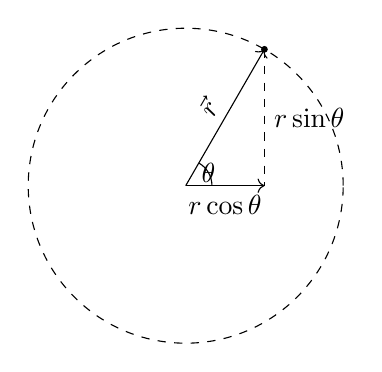
\begin{tikzpicture}[scale=2]

            % draw the circle
            \draw[dashed] (0,0) circle (1);
            
            % draw the point on the circle
            \filldraw[black] ({cos(60)},{sin(60)}) circle (.5pt);
            
            % draw the vector
            \draw[->] (0,0) -- ({cos(60)},{sin(60)}) node[midway,above,sloped] {$\vec{r}$};
            
            % draw dashed line from point to x axis
            \draw[dashed] ({cos(60)},{sin(60)}) -- ({cos(60)},0);
            
            %label component r*sin(theta)
            \node[right] at ({cos(60)}, {sin(60)/2}) {$r\sin\theta$};
            
            % draw line from center to x coordinate of point
            \draw[->] (0,0) -- ({cos(60)},0);
            
            %label component r*cos(theta)
            \node[below] at ({cos(60)/2}, 0) {$r\cos\theta$};
            
            % draw arc for angle from horizontal component to vector
            \draw[-] ({cos(60)/3},0) arc (0:60:{cos(60)/3}) node[midway] {$\theta$};
            \end{tikzpicture}
    \end{figure}
    We can express the position vector in terms of the angle $\theta$:
    \begin{equation}
        \vec{r} = \begin{pmatrix} r\cos\theta \\ r\sin\theta \end{pmatrix}
    \end{equation}
    To express this position equation in terms of time for an object moving at constant speed, we make the substitution $\theta = \omega t + \theta_0$:
    \begin{equation}
        \vec{r} = \begin{pmatrix} r\cos(\omega t + \theta_0) \\ r\sin(\omega t + \theta_0) \end{pmatrix}
    \end{equation}
    Because the motion is uniform, the angle $\theta$ changes at a constant rate given by $\omega$ (the \textbf{angular velocity}) according to the equation $\omega = \frac{d\theta}{dt}$. $\theta_0$ is the initial angle of the object.
    \\
    \\
    We can differentiate the position vector to find the velocity vector:
    \begin{equation}
        \vec{v} = \omega r \begin{pmatrix} -\sin(\omega t + \theta_0) \\ \cos(\omega t + \theta_0) \end{pmatrix}
    \end{equation}
    \textbf{Direction of the Velocity Vector}: We can take the dot product of the velocity vector with the position vector to find the direction of the velocity vector:
    \begin{equation}
        \vec{r} \cdot \vec{v} = r_x v_x + r_y v_y = 0
    \end{equation}
    This indicates that the velocity vector is perpendicular to the position vector, which is what we expect, as the velocity is always tangent to the path of the particle, which in this case is tangent to the circle and thus perpendicular to the position vector.
    \\
    \\
    \textbf{Magnitude of the Velocity Vector}: 
    \begin{equation}
        ||\vec{v}|| = \sqrt{v_x^2 + v_y^2} = \omega r
        \label{eq:angular_velocity}
    \end{equation}
    We can differentiate the velocity vector to find the acceleration vector:
    \begin{equation}
        \vec{a} = -\omega^2 r \begin{pmatrix} \cos(\omega t + \theta_0) \\ \sin(\omega t + \theta_0) \end{pmatrix}
    \end{equation}
    \textbf{Direction of the Acceleration Vector}: From inspection, we see that $\vec{a}(t) = -\omega^2 \vec{r}(t)$. Because $\omega^2$ is positive, this equation implies that the acceleration vector is antiparallel to the position vector. Because the position vector points outward, the acceleration vector points inward, toward the center of rotation. This is why the acceleration is called \textbf{centripetal acceleration}.
    \\
    \\
    \textbf{Magnitude of the Acceleration Vector}:
    \begin{equation}
        ||\vec{a}|| = \sqrt{a_x^2 + a_y^2} = \omega^2 r
    \end{equation}
    Using \autoref{eq:angular_velocity}, we can write:
    \begin{equation}
        ||\vec{a}|| = \frac{v^2}{r}
    \end{equation}
\end{document}